\Titelbanner{10}{Integralrechnung}

\textbf{Aufgabe 1: } \emph{Stammfunktionen} \hfill Ziel: (a) bis (d)\\[0.2cm]
Bestimmen Sie jeweils die Stammfunktion $F(x)$ der folgenden Funktionen.
\begin{align*}
    &\text{(a)}\quad f(x)=\sin(2x+5)                && \text{(b)}\quad f(x)=\frac{k}{kx+1}\\[1ex]
    &\text{(c)}\quad f(x)=\frac{\cos(x)}{\sin(x)}	&& \text{(d)}\quad f(x)=\frac{a\cos(x)+b\sin(x)}{c\sin(x)}\\[1ex]
    &\text{(e)}\quad f(x)=\frac{x^2+1}{x^2-1}       && \text{(f)}\quad f(x)=\frac{kx}{\sqrt{x^2+y^2}^3}
\end{align*}    
\emph{Hinweis:} Partialbruchzerlegung in (e).\\[1cm]
%
\textbf{Aufgabe 2: } \emph{Partielle Integration}\hfill Ziel: (a) bis (c)\\[0.2cm]
Bestimmen Sie die folgenden Integrale unter Verwendung partieller Integration.
\begin{align*}
    &\text{(a)}\quad \int\limits_0^\pi x\sin(x)\dd{x}	&& \text{(b)}\quad \int\limits_0^1 x^3\e^{x}\dd{x}\\[1ex]
    &\text{(c)}\quad \int\limits_{r_0}^{2r_0} r\qty(1+\ln\frac{r}{r_0})\dd{r}	&& \text{(d)}\quad \int\frac{\ln(x)}{x}\dd{x}
\end{align*}\\[0.8cm]
%
\textbf{Aufgabe 3: } \emph{Substitutionen}\\[0.2cm]
Berechnen Sie die folgenden Integrale jeweils unter Verwendung der angegebenen Substitution.
\begin{align*}
    &\text{(a)}\quad \int\limits_0^1 \sqrt{1-x^2}\dd{x}\,,		&&\text{mit}\quad x=\sin\phi\\[1ex]
    &\text{(b)}\quad \int\limits_0^1 \frac{\dd{x}}{(1+x^2)\sqrt{\arctan(x)}}	\,,	&&\text{mit}\quad u=\arctan(x)
\end{align*}
%

\newpage\noindent
\textbf{Aufgabe 4: } \emph{Vollständige Induktion} \hfill (Zusatzaufgabe)\\[0.2cm]
Zeigen Sie mithilfe vollständiger Induktion, dass für die Fakultät
\begin{align*}
        n! = \int\limits_{0}^{\infty} x^n \e^{-x} \dd{x},
\end{align*}
gilt. \emph{Hinweis}: Es gilt $0! = 1$.

\textbf{Aufgabe 5: } \emph{Flächenintegral}\\[0.2cm]
Leiten Sie die Formel für den Flächeninhalt eines Kreises vom Radius $R$ her.
\begin{center}
    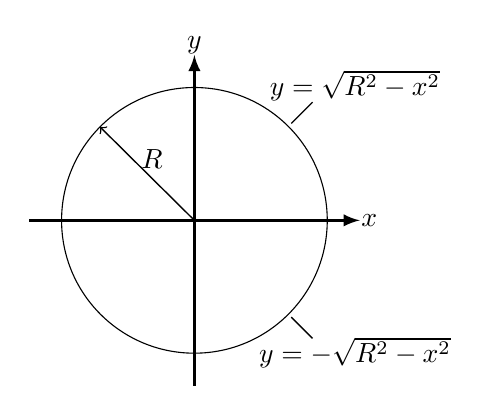
\begin{tikzpicture}[scale=0.6]
    \draw[-{latex}, line width=1pt] (0,-3.5)--(0,3.5);
    \draw[-{latex}, line width=1pt] (-3.5,0)--(3.5,0);
    \draw (0,0) circle (80pt);
    \node at (0,3.7) {$y$};
    \node at (3.7,0) {$x$};
    \draw[line width=0.5pt] (2.05,2.05)--(2.5,2.5);
    \draw[line width=0.5pt] (2.05,-2.05)--(2.5,-2.5);
    \node at (3.4,2.85) {$y=\sqrt{R^2-x^2}$};
    \node at (3.4,-2.8) {$y=-\sqrt{R^2-x^2}$};
    \draw[->,line width=0.5pt] (0,0)--(-2,1.98);
    \node at (-0.9,1.3) {$R$};
    \end{tikzpicture}
\end{center}
% \vspace{1cm}
%
\textbf{Aufgabe 6: } \emph{Volumenintegral} \hfill (Zusatzaufgabe)\\[0.2cm]
Berechnen Sie das Volumen des in der Abbildung gezeigten Körpers.
% \begin{center}
% \includegraphics[width=8cm]{koerper.pdf}
% \end{center}

\begin{figure}[htp]
    \centering
    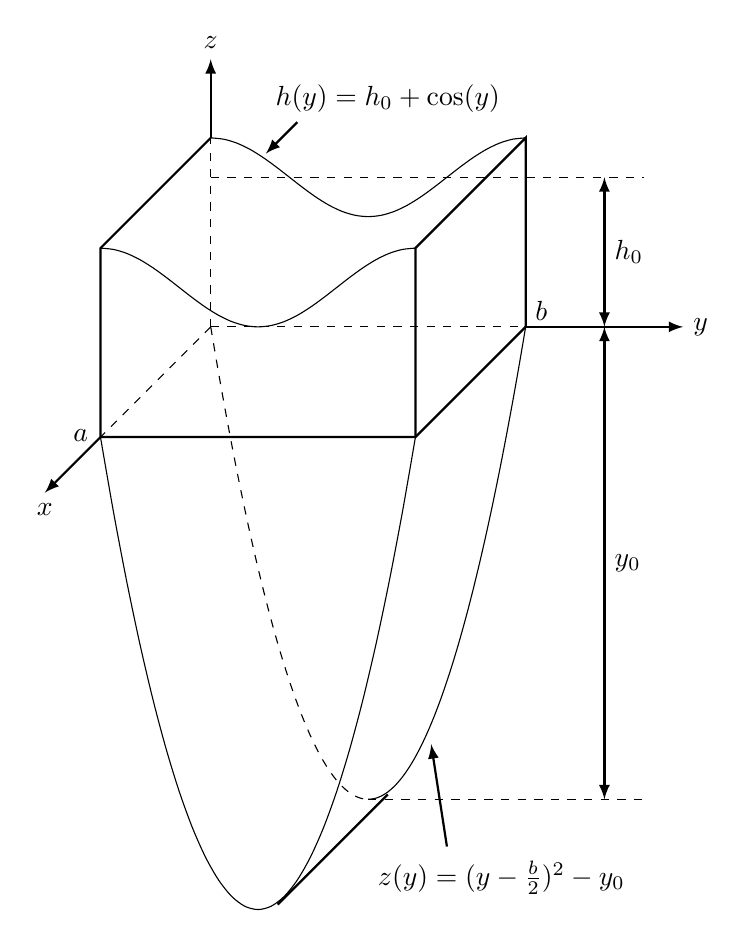
\begin{tikzpicture}
        \draw[dashed] (0,0) -- (-1.4,-1.4);
        \draw[dashed] (0,0) -- (0,2.4);
        \draw[dashed] (0,0) -- (4,0);
        \draw[thick,-{latex}] (-1.4,-1.4) -- +(-0.707,-0.707)node[below]{$x$};
        \draw[thick,-{latex}] (4,0) -- +(2,0)node[right]{$y$};
        \draw[thick,-{latex}] (0,2.4) -- +(0,1)node[above]{$z$};
        \draw[thick] (2+0.25,-6+0.0625) -- +(-1.4,-1.4);
        \draw[thick] (-1.4,-1.4) -- ++(4,0) -- ++(1.4,1.4);
        \draw[dashed] (0,1.9) -- +(5.5,0);
        \draw[dashed] (2,-6) -- +(3.5,0);
        \draw[thick, {latex}-{latex}] (5,1.9) --node[right]{$h_0$} (5,0);
        \draw[thick, {latex}-{latex}] (5,0) --node[right]{$y_0$} (5,-6);
        \node (A) at (-1.4-.25,-1.38){$a$};
        \node (A) at (4.2,0.2){$b$};
        \draw[ domain=2:4, smooth, variable=\x] plot ({\x}, {1.5*(\x-2)*(\x-2)-6});
        \draw[ domain=0:2, dashed, smooth, variable=\x] plot ({\x}, {1.5*(\x-2)*(\x-2)-6});
        \draw[ domain=-1.4:2.6, smooth, variable=\x] plot ({\x}, {1.5*(\x-0.6)*(\x-0.6)-6-1.4});
        \draw[ domain=-1.4:2.6, smooth, variable=\x] plot ({\x}, {0.5*cos(deg((\x+1.4)*3.1415/2))+0.5});
        \draw[ domain=0:4, smooth, variable=\x] plot ({\x}, {0.5*cos(deg((\x)*3.1415/2))+0.5+1.4});
        \draw[thick] (-1.4,-1.4) -- ++(0,2.4) -- ++(1.4,1.4);
        \draw[thick] (2.6,-1.4) -- ++(0,2.4) -- ++(1.4,1.4) -- ++(0,-2.4);
        \node[anchor=west] at (0.7,2.9){$h(y)=h_0 + \cos(y) $};
        \draw[thick, -{latex}] (1.1,2.6) --+(-0.4,-.4);
        \node[anchor=west] at (2,-7){$z(y) = \qty(y-\frac{b}{2})^2 - y_0 $};
        \draw[thick, -{latex}] (3,-6.6) --+(-.2,1.3);
    \end{tikzpicture}
\end{figure}
